%%%%%%%%%%%%%%%%%%%%%%%%%%%%%%%%%%%%%%%%%%%%%%%%%%%%%%%%%%%%%%%%%%%%%%%%%%%%
% AGUtmpl.tex: this template file is for articles formatted with LaTeX2e,
% Modified November 2013
%
% This template includes commands and instructions
% given in the order necessary to produce a final output that will
% satisfy AGU requirements.
%
% PLEASE DO NOT USE YOUR OWN MACROS
% DO NOT USE \newcommand, \renewcommand, or \def.
%
% FOR FIGURES, DO NOT USE \psfrag
%
%%%%%%%%%%%%%%%%%%%%%%%%%%%%%%%%%%%%%%%%%%%%%%%%%%%%%%%%%%%%%%%%%%%%%%%%%%%%
%
% All questions should be e-mailed to latex@agu.org.
%
%%%%%%%%%%%%%%%%%%%%%%%%%%%%%%%%%%%%%%%%%%%%%%%%%%%%%%%%%%%%%%%%%%%%%%%%%%%%
%
% Step 1: Set the \documentclass
%
% There are two options for article format: two column (default)
% and draft.
%
% PLEASE USE THE DRAFT OPTION TO SUBMIT YOUR PAPERS.
% The draft option produces double spaced output.
%
% Choose the journal abbreviation for the journal you are
% submitting to:

% jgrga JOURNAL OF GEOPHYSICAL RESEARCH
% gbc   GLOBAL BIOCHEMICAL CYCLES
% grl   GEOPHYSICAL RESEARCH LETTERS
% pal   PALEOCEANOGRAPHY
% ras   RADIO SCIENCE
% rog   REVIEWS OF GEOPHYSICS
% tec   TECTONICS
% wrr   WATER RESOURCES RESEARCH
% gc    GEOCHEMISTRY, GEOPHYSICS, GEOSYSTEMS
% sw    SPACE WEATHER
% ms    JAMES
% ef    EARTH'S FUTURE
%
%
%
% (If you are submitting to a journal other than jgrga,
% substitute the initials of the journal for "jgrga" below.)

\documentclass[draft,ms]{agutexSI}

\usepackage{rotating}


% Author names in capital letters:
\authorrunninghead{HUANG ET AL.}

% Shorter version of title entered in capital letters:
\titlerunninghead{EVALUATION OF VR-CESM IN REGIONAL CLIMATE MODEL}

%Corresponding author mailing address and e-mail address:
%\authoraddr{Corresponding author: A. B. Smith,
%Department of Hydrology and Water Resources, University of
%Arizona, Harshbarger Building 11, Tucson, AZ 85721, USA.
%(a.b.smith@hwr.arizona.edu)}

\begin{document}

%% ------------------------------------------------------------------------ %%
%
%  TITLE
%
%% ------------------------------------------------------------------------ %%

%\includegraphics{agu_pubart-white_reduced.eps}


\title{Supporting Information for ``An Evaluation of the Variable Resolution-CESM for Modeling California's Climate''}

%% ------------------------------------------------------------------------ %%
%
%  BEGIN ARTICLE
%
%% ------------------------------------------------------------------------ %%

% The body of the article must start with a \begin{article} command
%
% \end{article} must follow the references section, before the figures
%  and tables.

\begin{article}

%% ------------------------------------------------------------------------ %%
%
%  TEXT
%
%% ------------------------------------------------------------------------ %%



\noindent\textbf{Contents of this file}
%%%Remove or add items as needed%%%
\begin{enumerate}
\item Figures S1 to S19
\item Tables S1 to S4
%if Tables are larger than 1 page, upload as separate excel file
\end{enumerate}
\ \\

\noindent\textbf{Additional Supporting Information (Files uploaded separately)}
\begin{enumerate}
\item VR-CESM 0.25$^\circ$ grid mesh file
\item VR-CESM 0.125$^\circ$ grid mesh file
\end{enumerate}
\ \\

\noindent\textbf{Introduction}


This supporting information includes:

\begin{itemize}
\item[1)] The original grid-refined mesh files describing the variable-resolution cubed-sphere grids;

\item[2)] The interannual variability plots of mean T$_{max}$, T$_{min}$, T$_{avg}$ and Pr in simulations and PRISM over 5, 10, 20 and 25 years.  These plots show that our simulation period from year 1980-2005 is appropriate for the regional climatology studies in this paper;

\item[3)] Figures depicting the spatial distribution of T$_{max}$, T$_{min}$, T$_{avg}$ and Pr trends in models and PRISM over the period 1980-2005, including the indicator of statistical significance under the two-tailed t-statistic with a significance level of 0.05;

\item[4)] Plots of seasonally-averaged T$_{max}$, T$_{min}$, and T$_{avg}$ for seasons not addressed in this paper, and associated tabulated statistics;

\item[5)] Results from a globally uniform CESM run at 0.25$^\circ$ spatial resolution with the finite volume (FV) dynamical core \citep{wehner2014effect}.
\end{itemize}


%%% End of body of article:
%%%%%%%%%%%%%%%%%%%%%%%%%%%%%%%%%%%%%%%%%%%%%%%%%%%%%%%%%%%%%%%%
%
% Optional Notation section goes here
%
% Notation -- End each entry with a period.
% \begin{notation}
% Term & definition.\\
% Second term & second definition.\\
% \end{notation}
%%%%%%%%%%%%%%%%%%%%%%%%%%%%%%%%%%%%%%%%%%%%%%%%%%%%%%%%%%%%%%%%


%% ------------------------------------------------------------------------ %%
%%  REFERENCE LIST AND TEXT CITATIONS
%
% Either type in your references using
\begin{thebibliography}{1}
\providecommand{\natexlab}[1]{#1}
\expandafter\ifx\csname urlstyle\endcsname\relax
  \providecommand{\doi}[1]{doi:\discretionary{}{}{}#1}\else
  \providecommand{\doi}{doi:\discretionary{}{}{}\begingroup
  \urlstyle{rm}\Url}\fi
  
\bibitem[{\textit{Wehner et~al.}(2014)\textit{Wehner, Reed, Li, Prabhat,
  Bacmeister, Chen, Paciorek, Gleckler, Sperber, Collins, Gettelman, and
  Jablonowski}}]{wehner2014effect}
Wehner, M.~F., K.~Reed, F.~Li, Prabhat, J.~Bacmeister, C.-T. Chen, C.~Paciorek,
  P.~Gleckler, K.~Sperber, W.~D. Collins, A.~Gettelman, and C.~Jablonowski
  (2014), {The effect of horizontal resolution on simulation quality in the
  Community Atmospheric Model, CAM5.1}, \textit{J. Model. Earth. Sys.},
  \doi{10.1002/2013MS000276}.
  
\end{thebibliography}
%% ------------------------------------------------------------------------ %%
%
%  END ARTICLE
%
%% ------------------------------------------------------------------------ %%
\end{article}
\clearpage

 
\begin{figure}
\setfigurenum{S1}
\begin{center}
\includegraphics[width=6in]{SampleStd_annual_Tmax_80-04.pdf}
\caption{Sample standard deviation of annual T$_{max}$ from models and PRISM with 5 year step from year 1980.}
\end{center}
\end{figure}

\begin{figure}
\setfigurenum{S2}
\begin{center}
\includegraphics[width=6in]{SampleStd_annual_Tmin_80-04.pdf}
\caption{Sample standard deviation of annual T$_{min}$ from models and PRISM with 5 year step from year 1980.}
\end{center}
\end{figure}

\begin{figure}
\setfigurenum{S3}
\begin{center}
\includegraphics[width=6in]{SampleStd_annual_Tavg_80-04.pdf}
\caption{Sample standard deviation of annual T$_{avg}$ from models and PRISM with 5 year step from year 1980.}
\end{center}
\end{figure}

\begin{figure}
\setfigurenum{S4}
\begin{center}
\includegraphics[width=6in]{SampleStd_annual_Pr_80-04.pdf}
\caption{Sample standard deviation of annual Pr from models and PRISM with 5 year step from year 1980.}
\end{center}
\end{figure}

\begin{figure}
\setfigurenum{S5}
\begin{center}
\includegraphics[width=6in]{SampleStd_JJA_Tmax_80-04.pdf}
\caption{Sample standard deviation of JJA T$_{max}$ from models and PRISM with 5 year step from year 1980.}
\end{center}
\end{figure}

\begin{figure}
\setfigurenum{S6}
\begin{center}
\includegraphics[width=6in]{SampleStd_JJA_Tmin_80-04.pdf}
\caption{Sample standard deviation of JJA T$_{min}$ from models and PRISM with 5 year step from year 1980.}
\end{center}
\end{figure}

\begin{figure}
\setfigurenum{S7}
\begin{center}
\includegraphics[width=6in]{SampleStd_JJA_Tavg_80-04.pdf}
\caption{Sample standard deviation of JJA T$_{avg}$ from models and PRISM with 5 year step from year 1980.}
\end{center}
\end{figure}

\begin{figure}
\setfigurenum{S8}
\begin{center}
\includegraphics[width=6in]{SampleStd_DJF_Pr_80-04.pdf}
\caption{Sample standard deviation of DJF Pr from models and PRISM with 5 year step from year 1980.}
\end{center}
\end{figure}

\begin{figure}
\setfigurenum{S9}
\begin{center}
\includegraphics[width=6in]{Ttest_AnnualT2_timeTrend_over_1980-2005.pdf}
\caption{Results of Student's t-test for a statistically significant linear time trend of annual T$_{max}$, T$_{min}$ and T$_{avg}$ over 1980-2005 of models and PRISM.}
\end{center}
\end{figure}

\begin{figure}
\setfigurenum{S10}
\begin{center}
\includegraphics[width=6in]{Ttest_JJAT2_timeTrend_over_1980-2005.pdf}
\caption{Results of Student's t-test for a statistically significant linear time trend of JJA T$_{max}$, T$_{min}$ and T$_{avg}$ over 1980-2005 of models and PRISM.}
\end{center}
\end{figure}

\begin{figure}
\setfigurenum{S11}
\begin{center}
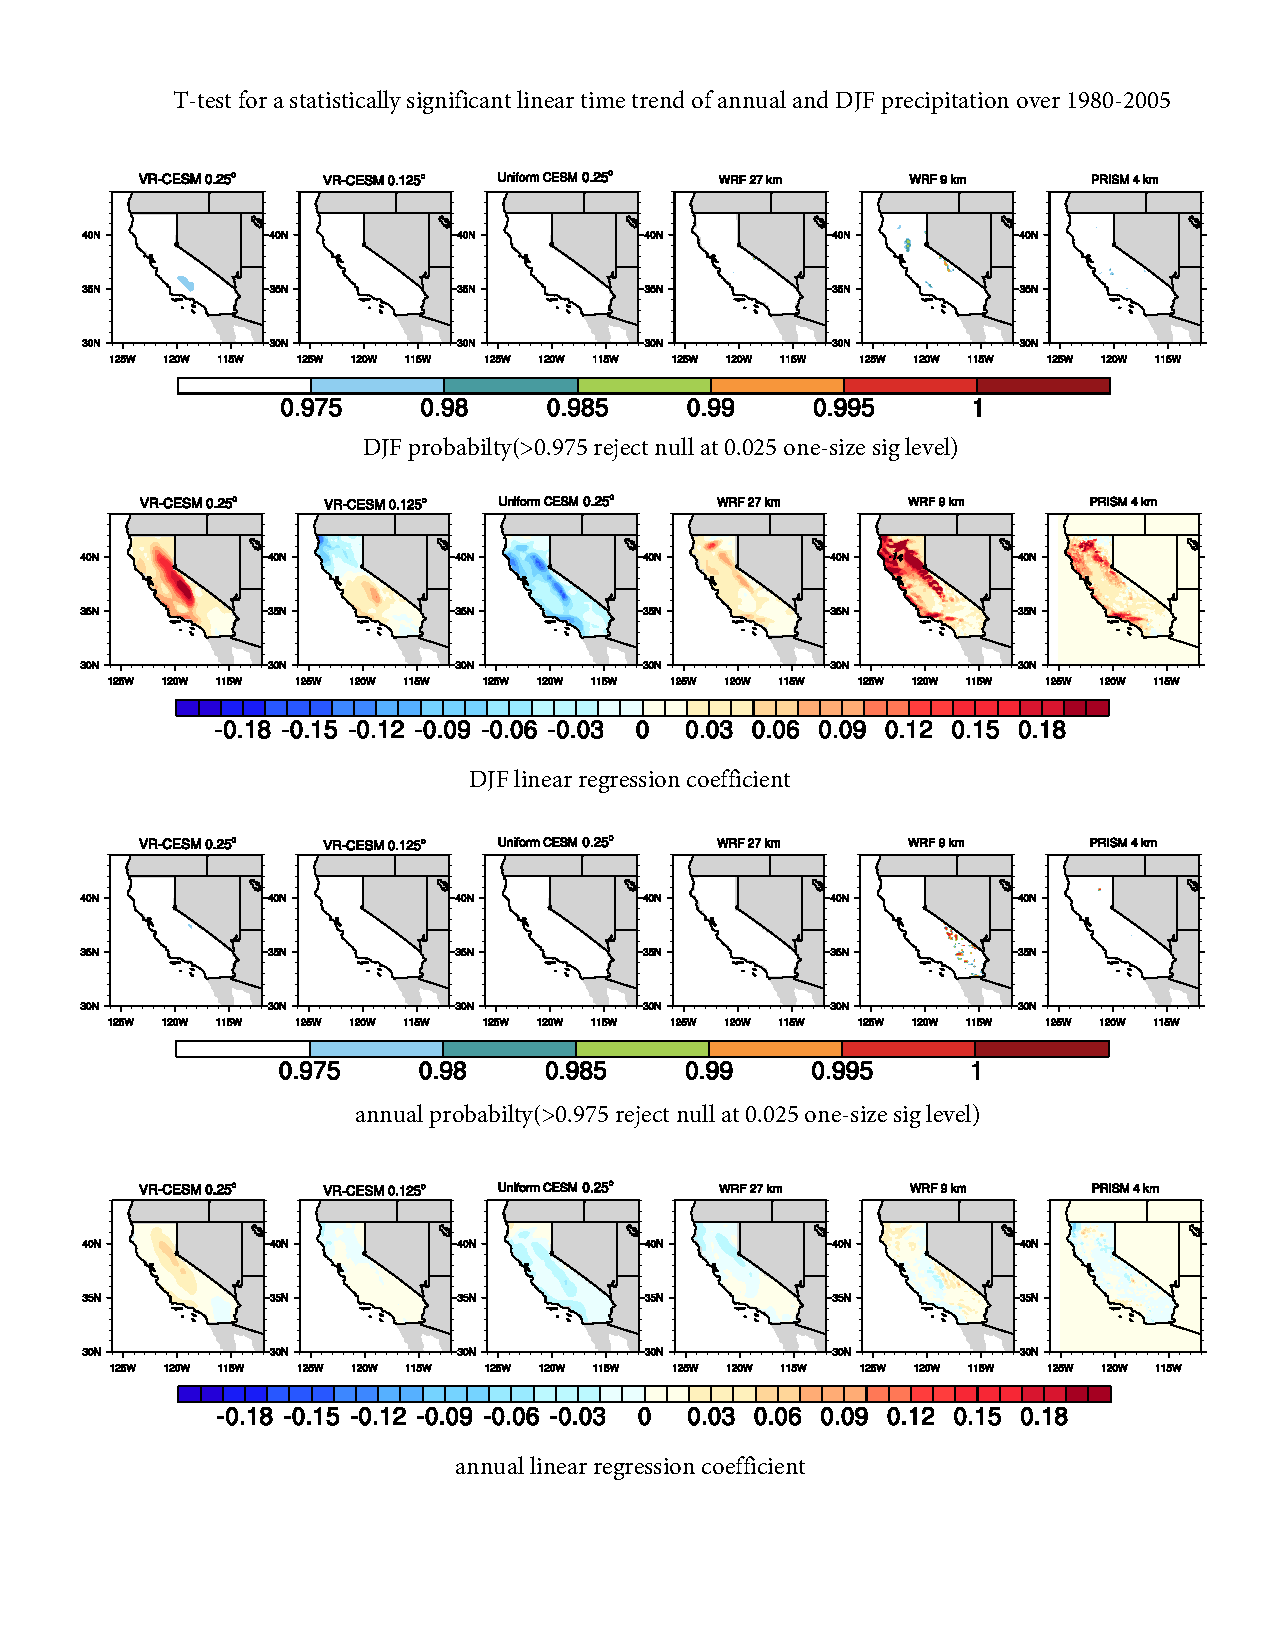
\includegraphics[width=6in]{Ttest_precipitation_timeTrend_over_1980-2005.pdf}
\caption{Results of Student's t-test for a statistically significant linear time trend of annual and DJF precipitation over 1980-2005 of models and PRISM.}
\end{center}
\end{figure}

\begin{figure}
\setfigurenum{S12}
\begin{center}
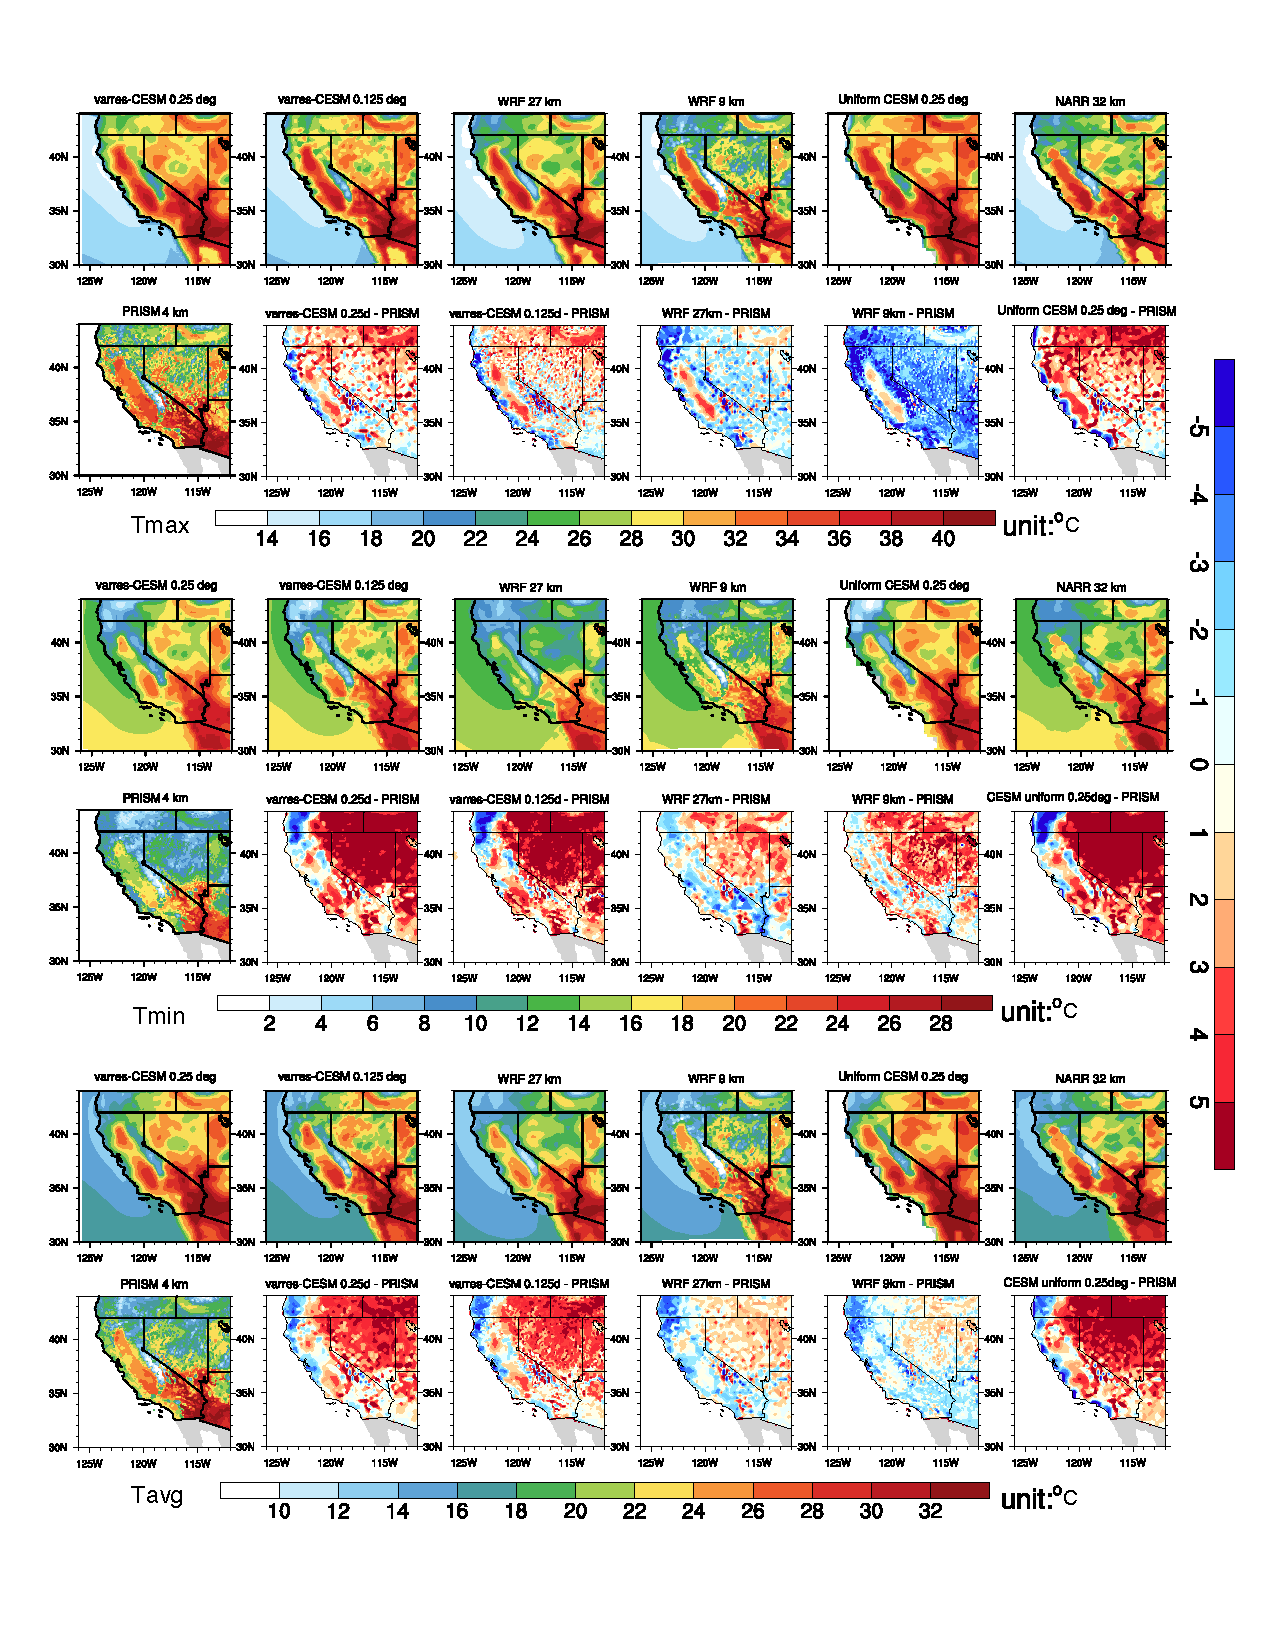
\includegraphics[width=6in]{t2_JJA_with_uniform_CESM.pdf}
\caption{Same as Figure 4 for season JJA along with uniform CESM 0.25$^\circ$.}
\end{center}
\end{figure}

\begin{figure}
\setfigurenum{S13}
\begin{center}
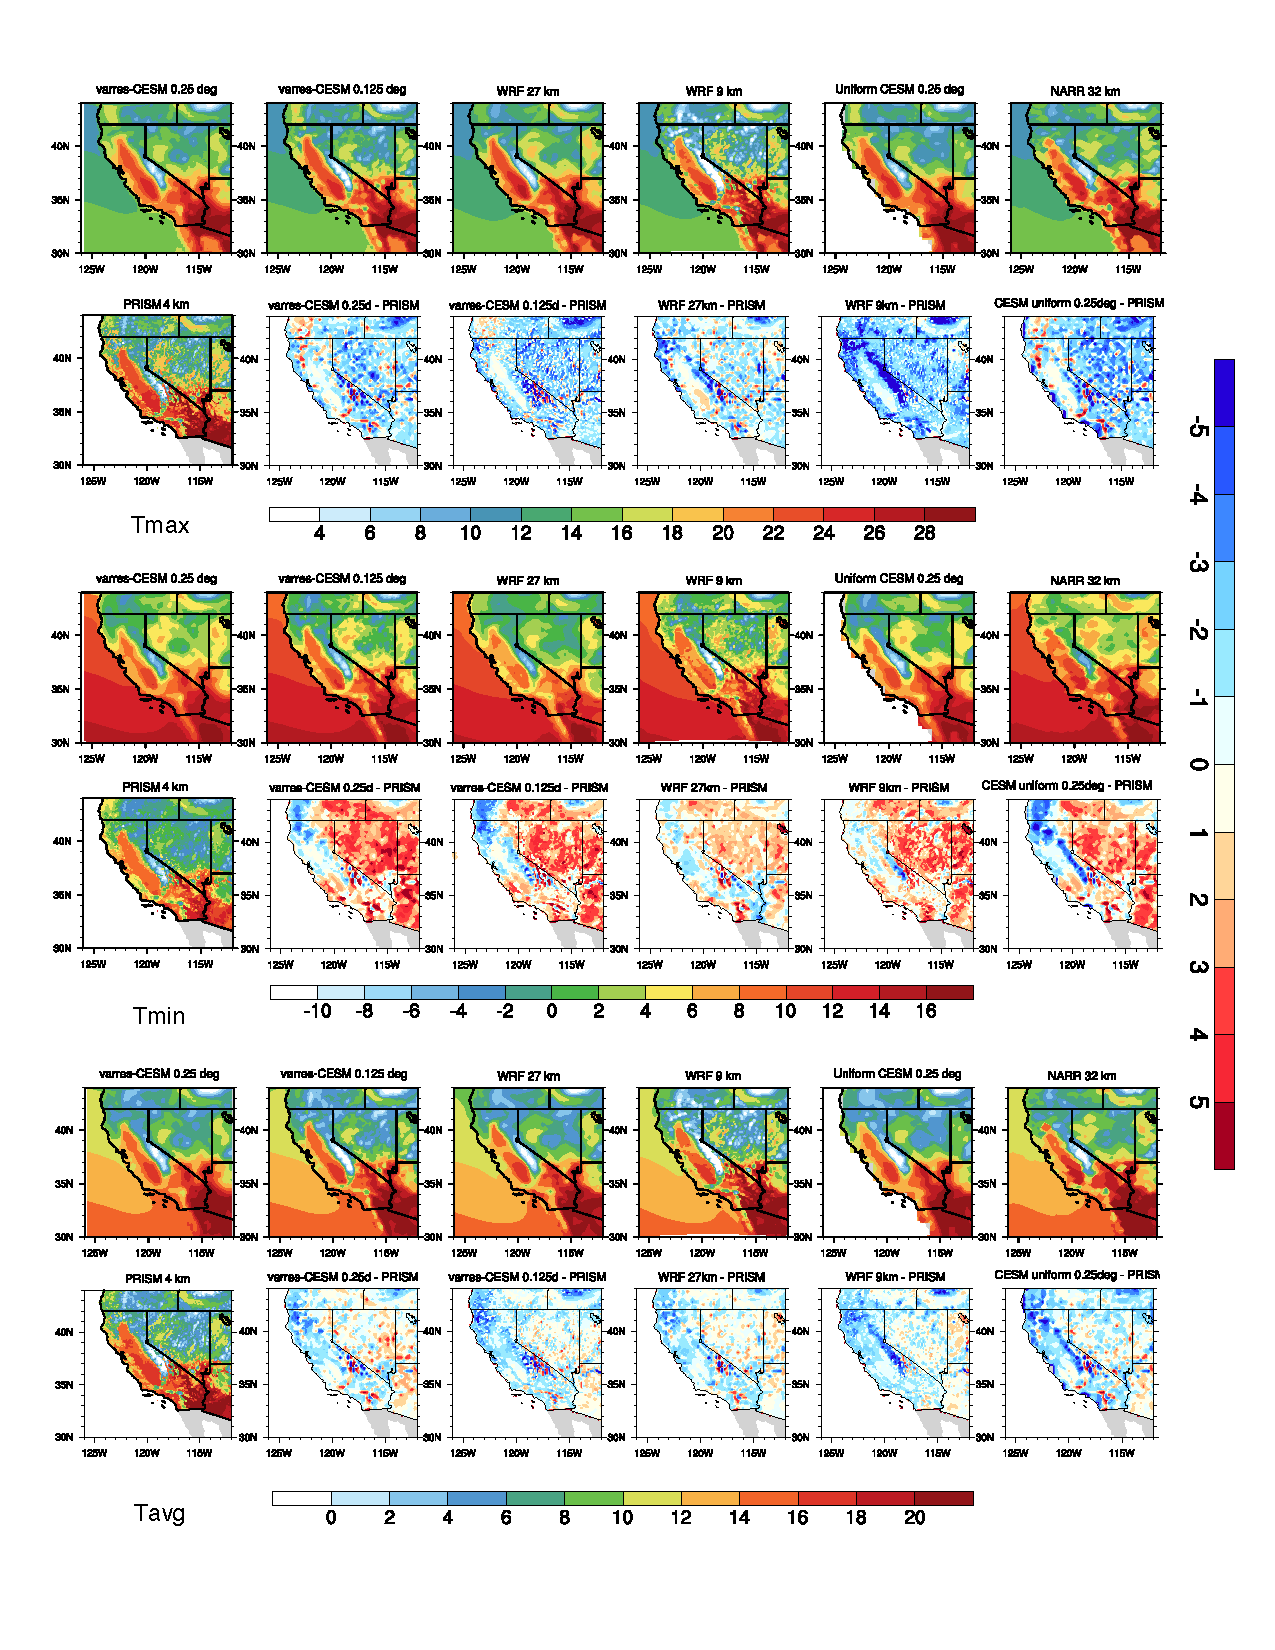
\includegraphics[width=6in]{t2_MAM.pdf}
\caption{As Figure 4 for season MAM along with uniform CESM 0.25$^\circ$.}
\end{center}
\end{figure}

\begin{figure}
\setfigurenum{S14}
\begin{center}
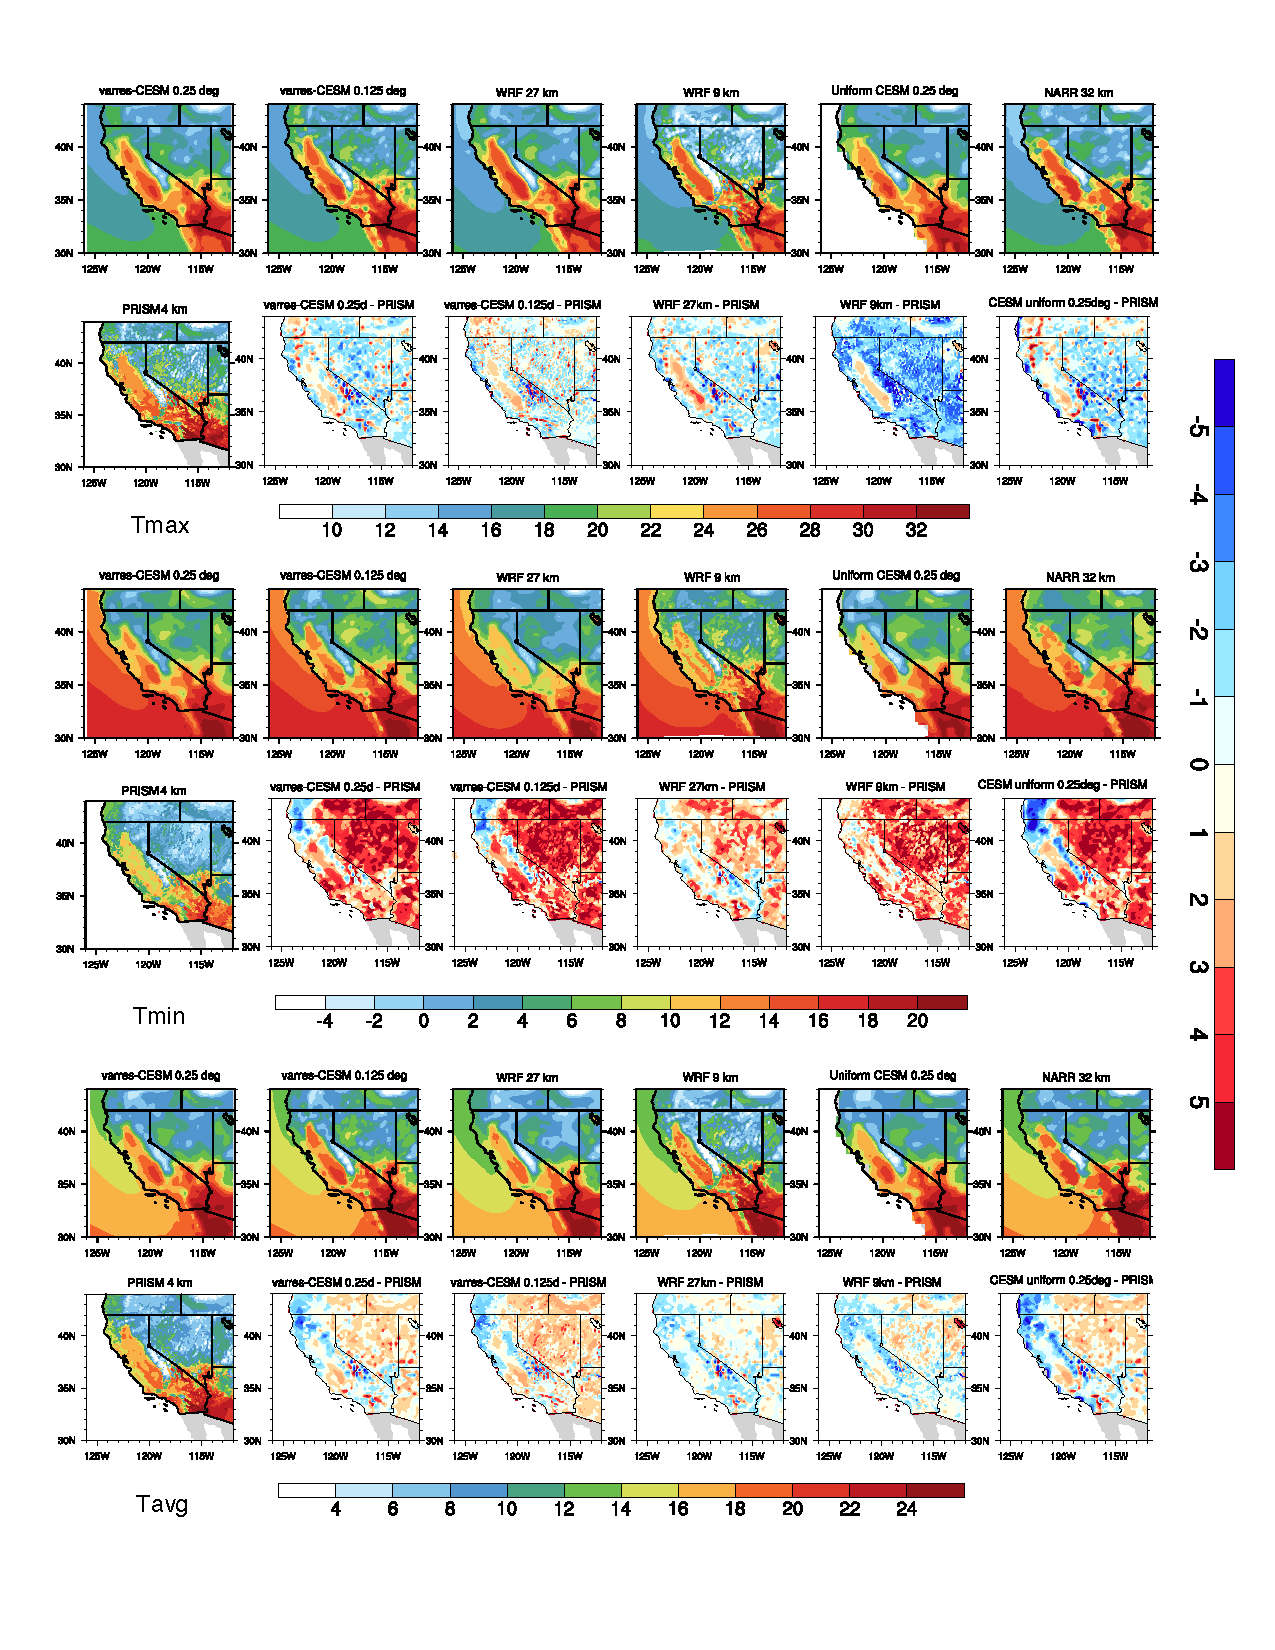
\includegraphics[width=6in]{t2_SON.pdf}
\caption{As Figure 4 for season SON along with uniform CESM 0.25$^\circ$.}
\end{center}
\end{figure}

\begin{figure}
\setfigurenum{S15}
\begin{center}
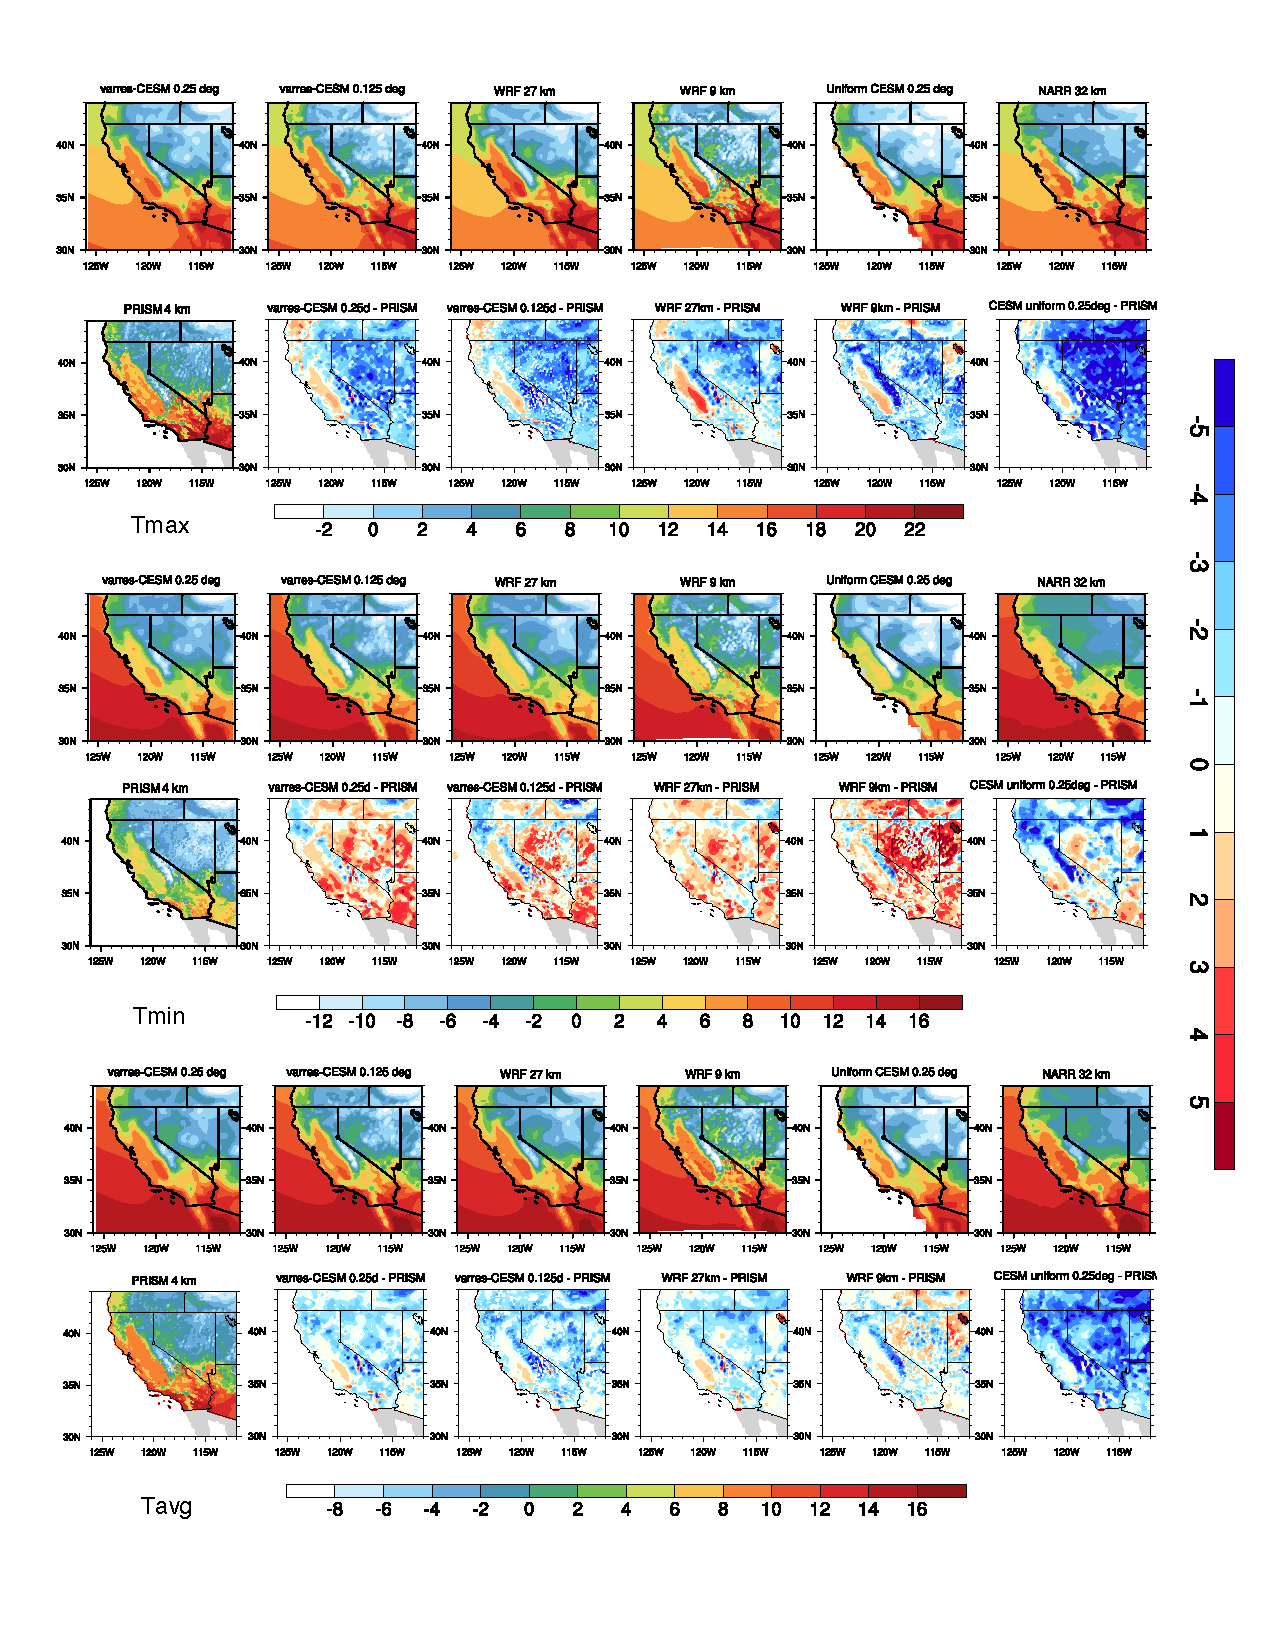
\includegraphics[width=6in]{t2_DJF.pdf}
\caption{As Figure 4 for season DJF along with uniform CESM 0.25$^\circ$.}
\end{center}
\end{figure}

\begin{figure}
\setfigurenum{S16}
\begin{center}
\includegraphics[width=6in]{trd_t2avg_allzones_with_uniform_CESM.pdf}
\caption{As Figure 6 but with the addition of uniform CESM 0.25$^\circ$.}
\end{center}
\end{figure}

\begin{figure}
\setfigurenum{S17}
\begin{center}
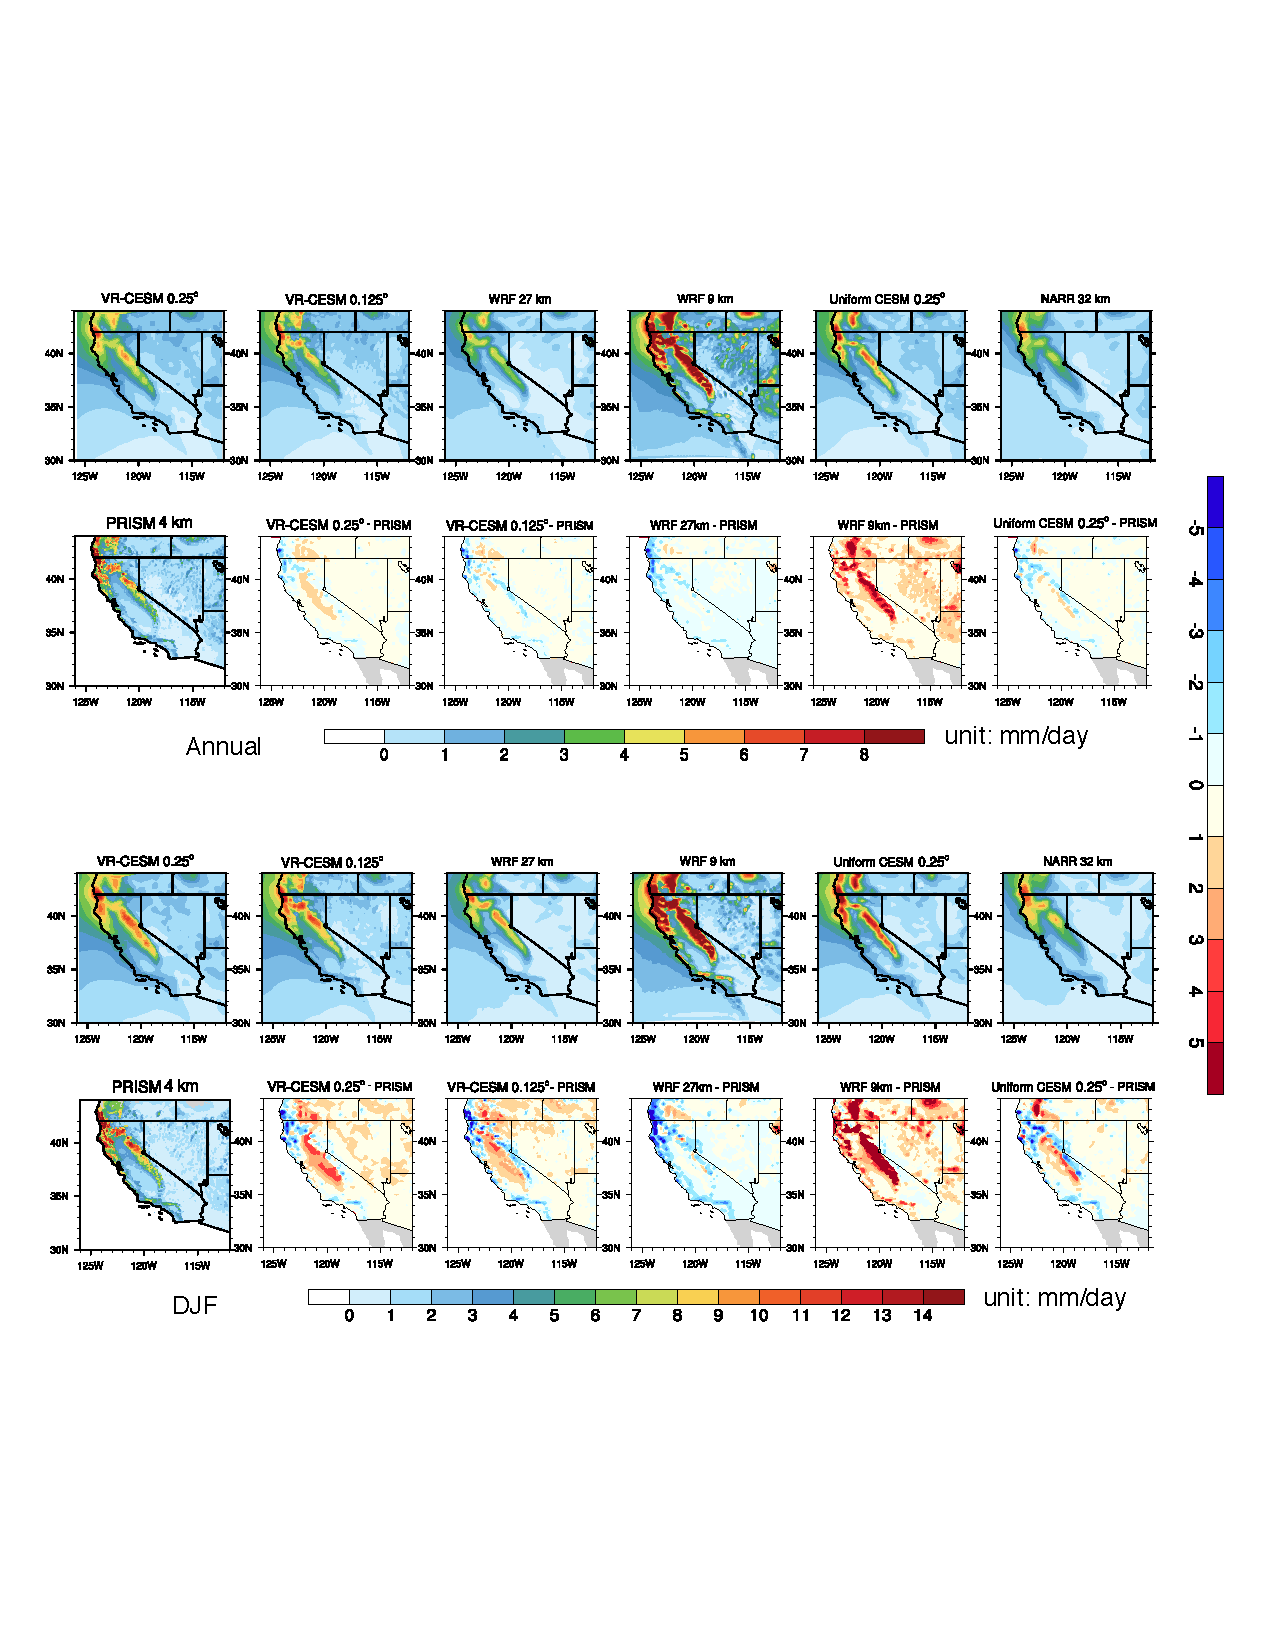
\includegraphics[width=6in]{pr_DJF_Annual_with_uniform_CESM.pdf}
\caption{As Figure 9 but with the addition of uniform CESM 0.25$^\circ$.}
\end{center}
\end{figure}

\begin{figure}
\setfigurenum{S18}
\begin{center}
\includegraphics[width=6in]{trd_pr_allzones_with_uniform_CESM.pdf}
\caption{As Figure 11 but with the addition of uniform CESM 0.25$^\circ$.}
\end{center}
\end{figure}

\clearpage

\begin{figure}
\setfigurenum{S19}
\begin{center}
\includegraphics[width=6in]{taylor_diagram_with_uniform_CESM.pdf}
\caption{As Figure 14 but with the addition of uniform CESM 0.25$^\circ$.}
\end{center}
\end{figure}

\clearpage


%%%%%Table 1%%%%%%%%%
\begin{table}
\settablenum{S1}
\begin{center}
\caption{RMSD ($^\circ C$), MSD ($^\circ C$) and Spatial Correlation (Corr) for seasonally-averaged MAM (March-April-May) temperature over California} 
\begin{tabular}{lcccc}
\hline \textbf{RMSD} & \textbf{UW}  & \textbf{PRISM} & \textbf{Daymet} \\
\hline $    $ & T$_{max}$ $\     $  T$_{min}$ & T$_{max}$ $\     $  T$_{min}$ $\     $ T$_{avg}$& T$_{max}$ $\     $  T$_{min}$\\
\hline \textbf{VR-CESM 0.25$^\circ$} & 1.776 $\ $ 2.212 & 2.297 $\ $ 2.164 $\ $ 2.033 & 2.344 $\ $ 2.686 \\
\textbf{VR-CESM 0.125$^\circ$} & 1.727 $\ $ 1.841 & 2.145 $\ $ 1.883 $\ $ 1.908 & 2.214 $\ $ 2.287 \\
\textbf{WRF 27km} & 1.945 $\ $ 2.062 & 2.433 $\ $ 1.863 $\ $ 1.991 & 2.366 $\ $ 2.541 \\
\textbf{WRF 9km} & 3.114 $\ $ 2.065 & 3.060 $\ $ 1.568 $\ $ 1.801 & 2.969 $\ $ 2.293 \\
\textbf{Uniform CESM 0.25$^\circ$} & 2.680 $\ $ 2.112 & 3.059 $\ $ 2.404 $\ $ 2.674 & 3.099 $\ $ 2.631 \\
\hline
\\
\end{tabular}

\begin{tabular}{lcccc}
\hline \textbf{MSD} & \textbf{UW}  & \textbf{PRISM} & \textbf{Daymet} \\
\hline $    $ & T$_{max}$ $\     $  T$_{min}$ & T$_{max}$ $\     $  T$_{min}$ $\     $ T$_{avg}$& T$_{max}$ $\     $  T$_{min}$\\
\hline \textbf{VR-CESM 0.25$^\circ$} & -0.859 $\ $ 1.308 & -0.813 $\ $ 0.681 $\ $ -0.819 & -0.608 $\ $ 1.350 \\
\textbf{VR-CESM 0.125$^\circ$} & -1.261 $\ $ 0.983 & -1.274 $\ $ 0.328 $\ $ -1.202 & -1.052 $\ $ 0.952 \\
\textbf{WRF 27km} & -1.066 $\ $ 0.745 & -1.020 $\ $ 0.117 $\ $ -0.942 & -0.818 $\ $ 0.788 \\
\textbf{WRF 9km} & -2.516 $\ $ 1.259 & -2.530 $\ $ 0.604 $\ $ -1.312 & -2.305 $\ $ 1.227 \\
\textbf{Uniform CESM 0.25$^\circ$} & -1.191 $\ $ 0.417 & -1.139 $\ $ -0.212 $\ $ -1.398 & -0.938 $\ $ 0.458 \\
\hline
\\
\end{tabular}

\begin{tabular}{lcccc}
\hline \textbf{Corr} & \textbf{UW}  & \textbf{PRISM} & \textbf{Daymet} \\
\hline $    $ & T$_{max}$ $\     $  T$_{min}$ & T$_{max}$ $\     $  T$_{min}$ $\     $ T$_{avg}$& T$_{max}$ $\     $  T$_{min}$\\
\hline \textbf{VR-CESM 0.25$^\circ$} & 0.997 $\ $ 0.963 & 0.995 $\ $ 0.963 $\ $ 0.990 & 0.994 $\ $ 0.942 \\
\textbf{VR-CESM 0.125$^\circ$} & 0.998 $\ $ 0.975 & 0.996 $\ $ 0.972 $\ $ 0.993 & 0.995 $\ $ 0.959 \\
\textbf{WRF 27km} & 0.996 $\ $ 0.959 & 0.994 $\ $ 0.968 $\ $ 0.991 & 0.994 $\ $ 0.937 \\
\textbf{WRF 9km} & 0.993 $\ $ 0.971 & 0.994 $\ $ 0.983 $\ $ 0.994 & 0.993 $\ $ 0.962 \\
\textbf{Uniform CESM 0.25$^\circ$} & 0.993 $\ $ 0.960 & 0.990 $\ $ 0.949 $\ $ 0.984 & 0.989 $\ $ 0.938 \\
\hline
\end{tabular}
\end{center}
\end{table}

%%%%%Table 2%%%%%%%%%
\begin{table}
\settablenum{S2}
\begin{center}
\caption{RMSD ($^\circ C$), MSD ($^\circ C$) and Spatial Correlation (Corr) for seasonally-averaged SON (Sept.-Oct.-Nov.) temperature over California.} 
\begin{tabular}{lcccc}
\hline \textbf{RMSD} & \textbf{UW}  & \textbf{PRISM} & \textbf{Daymet} \\
\hline $    $ & T$_{max}$ $\     $  T$_{min}$ & T$_{max}$ $\     $  T$_{min}$ $\     $ T$_{avg}$& T$_{max}$ $\     $  T$_{min}$\\
\hline \textbf{VR-CESM 0.25$^\circ$} & 1.591 $\ $ 3.866 & 2.065 $\ $ 2.788 $\ $ 1.777 & 2.088 $\ $ 3.837 \\
\textbf{VR-CESM 0.125$^\circ$} & 1.212 $\ $ 3.906 & 1.652 $\ $ 2.851 $\ $ 1.524 & 1.900 $\ $ 3.797 \\
\textbf{WRF 27km} & 1.665 $\ $ 3.022 & 2.111 $\ $ 1.784 $\ $ 1.663 & 2.059 $\ $ 3.060 \\
\textbf{WRF 9km} & 2.262 $\ $ 3.788 & 2.574 $\ $ 2.322 $\ $ 1.285 & 2.402 $\ $ 3.615 \\
\textbf{uniform CESM 0.25$^\circ$} & 2.605 $\ $ 3.344 & 2.970 $\ $ 2.789 $\ $ 2.464 & 2.999 $\ $ 3.444 \\
\hline
\\
\end{tabular}

\begin{tabular}{lcccc}
\hline \textbf{MSD} & \textbf{UW}  & \textbf{PRISM} & \textbf{Daymet} \\
\hline $    $ & T$_{max}$ $\     $  T$_{min}$ & T$_{max}$ $\     $  T$_{min}$ $\     $ T$_{avg}$& T$_{max}$ $\     $  T$_{min}$\\
\hline \textbf{VR-CESM 0.25$^\circ$} & 0.122 $\ $ 3.303 & -0.353 $\ $ 1.766 $\ $ -0.240 & 0.102 $\ $ 3.063 \\
\textbf{VR-CESM 0.125$^\circ$} & 0.394 $\ $ 3.439 & -0.126 $\ $ 1.908 $\ $ -0.048 & 0.353 $\ $ 3.134 \\
\textbf{WRF 27km} & 0.181 $\ $ 2.044 & -0.295 $\ $ 0.507 $\ $ -0.739 & 0.158 $\ $ 1.807 \\
\textbf{WRF 9km} & -1.412 $\ $ 3.310 & -1.931 $\ $ 1.779 $\ $ -0.673 & -1.451 $\ $ 3.004 \\
\textbf{uniform CESM 0.25$^\circ$} & -0.187 $\ $ 2.415 & -0.655 $\ $ 0.877 $\ $ -0.826 & -0.205 $\ $ 2.175 \\
\hline
\\
\end{tabular}

\begin{tabular}{lcccc}
\hline \textbf{Corr} & \textbf{UW}  & \textbf{PRISM} & \textbf{Daymet} \\
\hline $    $ & T$_{max}$ $\     $  T$_{min}$ & T$_{max}$ $\     $  T$_{min}$ $\     $ T$_{avg}$& T$_{max}$ $\     $  T$_{min}$\\
\hline \textbf{VR-CESM 0.25$^\circ$} & 0.998 $\ $ 0.950 & 0.996 $\ $ 0.975 $\ $ 0.994 & 0.996 $\ $ 0.951 \\
\textbf{VR-CESM 0.125$^\circ$} & 0.999 $\ $ 0.957 & 0.998 $\ $ 0.978 $\ $ 0.996 & 0.997 $\ $ 0.961 \\
\textbf{WRF 27km} & 0.997 $\ $ 0.949 & 0.996 $\ $ 0.982 $\ $ 0.995 & 0.996 $\ $ 0.948 \\
\textbf{WRF 9km} & 0.996 $\ $ 0.953 & 0.996 $\ $ 0.986 $\ $ 0.997 & 0.996 $\ $ 0.959 \\
\textbf{uniform CESM 0.25$^\circ$} & 0.993 $\ $ 0.956 & 0.992 $\ $ 0.965 $\ $ 0.989 & 0.991 $\ $ 0.952 \\
\hline
\\
\end{tabular}
\end{center}
\end{table}

%%%%%Table 3%%%%%%%%%
\begin{table}
\settablenum{S3}
\begin{center}
\caption{RMSD ($^\circ C$), MSD ($^\circ C$) and Spatial Correlation (Corr) for seasonally-averaged DJF temperature over California.} 
\begin{tabular}{lcccc}
\hline \textbf{RMSD} & \textbf{UW}  & \textbf{PRISM} & \textbf{Daymet} \\
\hline $    $ & T$_{max}$ $\     $  T$_{min}$ & T$_{max}$ $\     $  T$_{min}$ $\     $ T$_{avg}$& T$_{max}$ $\     $  T$_{min}$\\
\hline \textbf{VR-CESM 0.25$^\circ$} & 1.959 $\ $ 2.751 & 2.196 $\ $ 2.015 $\ $ 1.742 & 2.253 $\ $ 2.700 \\
\textbf{VR-CESM 0.125$^\circ$} & 1.633 $\ $ 2.302 & 2.035 $\ $ 1.840 $\ $ 1.747 & 2.089 $\ $ 2.318 \\
\textbf{WRF 27km} & 1.699 $\ $ 2.756 & 2.106 $\ $ 1.734 $\ $ 1.537 & 2.033 $\ $ 2.665 \\
\textbf{WRF 9km} & 1.876 $\ $ 2.753 & 2.324 $\ $ 1.865 $\ $ 1.324 & 2.169 $\ $ 2.625 \\
\textbf{uniform CESM 0.25$^\circ$} & 2.979 $\ $ 2.072 & 3.339 $\ $ 2.500 $\ $ 3.211 & 3.310 $\ $ 2.408 \\
\hline
\\
\end{tabular}

\begin{tabular}{lcccc}
\hline \textbf{MSD} & \textbf{UW}  & \textbf{PRISM} & \textbf{Daymet} \\
\hline $    $ & T$_{max}$ $\     $  T$_{min}$ & T$_{max}$ $\     $  T$_{min}$ $\     $ T$_{avg}$& T$_{max}$ $\     $  T$_{min}$\\
\hline \textbf{VR-CESM 0.25$^\circ$} & -0.549 $\ $ 2.108 & -0.984 $\ $ 0.977 $\ $ -0.920 & -0.774 $\ $ 1.836 \\
\textbf{VR-CESM 0.125$^\circ$} & -0.723 $\ $ 1.678 & -1.178 $\ $ 0.541 $\ $ -1.202 & -0.978 $\ $ 1.345 \\
\textbf{WRF 27km} & -0.075 $\ $ 2.027 & -0.510 $\ $ 0.895 $\ $ -0.620 & -0.302 $\ $ 1.759 \\
\textbf{WRF 9km} & -1.049 $\ $ 2.214 & -1.504 $\ $ 1.077 $\ $ -0.594 & -1.301 $\ $ 1.880 \\
\textbf{uniform CESM 0.25$^\circ$} & -1.862 $\ $ -0.010 & -2.293 $\ $ -1.142 $\ $ -2.616 & -2.085 $\ $ -0.280 \\
\hline
\\
\end{tabular}

\begin{tabular}{lcccc}
\hline \textbf{Corr} & \textbf{UW}  & \textbf{PRISM} & \textbf{Daymet} \\
\hline $    $ & T$_{max}$ $\     $  T$_{min}$ & T$_{max}$ $\     $  T$_{min}$ $\     $ T$_{avg}$& T$_{max}$ $\     $  T$_{min}$\\
\hline \textbf{VR-CESM 0.25$^\circ$} & 0.989 $\ $ 0.856 & 0.988 $\ $ 0.925 $\ $ 0.978 & 0.987 $\ $ 0.856 \\
\textbf{VR-CESM 0.125$^\circ$} & 0.993 $\ $ 0.900 & 0.991 $\ $ 0.941 $\ $ 0.979 & 0.989 $\ $ 0.898 \\
\textbf{WRF 27km} & 0.992 $\ $ 0.842 & 0.987 $\ $ 0.931 $\ $ 0.982 & 0.988 $\ $ 0.838 \\
\textbf{WRF 9km} & 0.990 $\ $ 0.859 & 0.987 $\ $ 0.942 $\ $ 0.987 & 0.988 $\ $ 0.870 \\
\textbf{uniform CESM 0.25$^\circ$} & 0.980 $\ $ 0.922 & 0.977 $\ $ 0.885 $\ $ 0.926 & 0.976 $\ $ 0.893 \\
\hline
\\
\end{tabular}
\end{center}
\end{table}


%%%%%Table 4%%%%%%%%%
\begin{table}
\settablenum{S4}
\begin{center}
\caption{RMSD (mm/day), MSD (mm/d), MRD, Spatial Correlation (Corr) for averaged precipitation over California}
\begin{tabular}{lcc}
\hline \textbf{MAM} & \textbf{CPC}  & \textbf{UW} \\
\hline $    $ & RMSD $\ $ MSD $\ $ MRD $\ $ Corr & RMSD $\ $ MSD $\ $ MRD $\ $ Corr \\
\hline \textbf{VR-CESM 0.25$^\circ$} & 0.542 $\ $ 0.279 $\ $ 0.264 $\ $ 0.981 & 0.589 $\ $ 0.193 $\ $ 0.265 $\ $ 0.968 \\
\textbf{VR-CESM 0.125$^\circ$} & 0.554 $\ $ 0.291 $\ $ 0.267 $\ $ 0.979 & 0.579 $\ $ 0.217 $\ $ 0.263 $\ $ 0.970\\
\textbf{WRF 27km} & 0.448 $\ $ -0.183 $\ $ 0.209 $\ $ 0.975 & 0.587 $\ $ -0.269 $\ $ 0.234 $\ $ 0.970 \\
\textbf{WRF 9km} & 2.143 $\ $ 1.370 $\ $ 0.881 $\ $ 0.966 & 1.991 $\ $ 1.295 $\ $ 0.783 $\ $ 0.971 \\
\textbf{uniform CESM 0.25$^\circ$} & 0.601 $\ $ 0.182 $\ $ 0.254 $\ $ 0.971 & 0.611 $\ $ 0.096 $\ $ 0.259 $\ $ 0.964 \\
\hline
\end{tabular}

\begin{tabular}{lcc}
\hline \textbf{MAM} & \textbf{PRISM} & \textbf{DAYMET} \\
\hline $    $ & RMSD $\ $ MSD $\ $ MRD $\ $ Corr & RMSD $\ $ MSD $\ $ MRD $\ $ Corr \\
\hline \textbf{VR-CESM 0.25$^\circ$} & 0.542 $\ $ 0.279 $\ $ 0.264 $\ $ 0.981 & 0.589 $\ $ 0.193 $\ $ 0.265 $\ $ 0.968 \\
\textbf{VR-CESM 0.125$^\circ$} & 0.554 $\ $ 0.291 $\ $ 0.267 $\ $ 0.979 & 0.579 $\ $ 0.217 $\ $ 0.263 $\ $ 0.970 \\
\textbf{WRF 27km} & 0.448 $\ $ -0.183 $\ $ 0.209 $\ $ 0.975 & 0.587 $\ $ -0.269 $\ $ 0.234 $\ $ 0.970 \\
\textbf{WRF 9km} & 2.143 $\ $ 1.370 $\ $ 0.881 $\ $ 0.966 & 1.991 $\ $ 1.295 $\ $ 0.783 $\ $ 0.971 \\
\textbf{uniform CESM 0.25$^\circ$} & 0.601 $\ $ 0.182 $\ $ 0.254 $\ $ 0.971 & 0.611 $\ $ 0.096 $\ $ 0.259 $\ $ 0.964 \\
\hline
\\
\end{tabular}

\begin{tabular}{lcc}
\hline \textbf{JJA} & \textbf{CPC}  & \textbf{UW} \\
\hline $    $ & RMSD $\ $ MSD $\ $ MRD $\ $ Corr & RMSD $\ $ MSD $\ $ MRD $\ $ Corr \\
\hline \textbf{VR-CESM 0.25$^\circ$} & 0.138 $\ $ -0.017 $\ $ 0.361 $\ $ 0.903 & 0.138 $\ $ -0.008 $\ $ 0.359 $\ $ 0.905 \\
\textbf{VR-CESM 0.125$^\circ$} & 0.153 $\ $ -0.006 $\ $ 0.388 $\ $ 0.889 & 0.148 $\ $ 0.005 $\ $ 0.375 $\ $ 0.897 \\
\textbf{WRF 27km} & 0.213 $\ $ 0.010 $\ $ 0.587 $\ $ 0.850 & 0.186 $\ $ 0.019 $\ $ 0.515 $\ $ 0.892 \\
\textbf{WRF 9km} & 1.013 $\ $ 0.644 $\ $ 2.518 $\ $ 0.853 & 1.000 $\ $ 0.654 $\ $ 2.654 $\ $ 0.881 \\
\textbf{uniform CESM 0.25$^\circ$} & 0.177 $\ $ -0.034 $\ $ 0.471 $\ $ 0.835 & 0.179 $\ $ -0.025 $\ $ 0.467 $\ $ 0.837 \\
\hline
\end{tabular}

\begin{tabular}{lcc}
\hline \textbf{JJA} & \textbf{PRISM} & \textbf{DAYMET} \\
\hline $    $ & RMSD $\ $ MSD $\ $ MRD $\ $ Corr & RMSD $\ $ MSD $\ $ MRD $\ $ Corr  \\
\hline \textbf{VR-CESM 0.25$^\circ$} & 0.138 $\ $ -0.017 $\ $ 0.361 $\ $ 0.903 & 0.138 $\ $ -0.008 $\ $ 0.359 $\ $ 0.905 \\
\textbf{VR-CESM 0.125$^\circ$} & 0.153 $\ $ -0.006 $\ $ 0.388 $\ $ 0.889 & 0.148 $\ $ 0.005 $\ $ 0.375 $\ $ 0.897 \\
\textbf{WRF 27km} & 0.213 $\ $ 0.010 $\ $ 0.587 $\ $ 0.850 & 0.186 $\ $ 0.019 $\ $ 0.515 $\ $ 0.892 \\
\textbf{WRF 9km} & 1.013 $\ $ 0.644 $\ $ 2.518 $\ $ 0.853 & 1.000 $\ $ 0.654 $\ $ 2.654 $\ $ 0.881 \\
\textbf{uniform CESM 0.25$^\circ$} & 0.177 $\ $ -0.034 $\ $ 0.471 $\ $ 0.835 & 0.179 $\ $ -0.025 $\ $ 0.467 $\ $ 0.837 \\
\hline
\\
\end{tabular}

\begin{tabular}{lcccc}
\hline \textbf{SON} & \textbf{CPC}  & \textbf{UW} \\
\hline $    $ & RMSD $\ $ MSD $\ $ MRD $\ $ Corr & RMSD $\ $ MSD $\ $ MRD $\ $ Corr \\
\hline \textbf{VR-CESM 0.25$^\circ$} & 0.536 $\ $ 0.346 $\ $ 0.338 $\ $ 0.984 & 0.579 $\ $ 0.323 $\ $ 0.351 $\ $ 0.966  \\
\textbf{VR-CESM 0.125$^\circ$} & 0.381 $\ $ -0.054 $\ $ 0.223 $\ $ 0.969 & 0.471 $\ $ -0.067 $\ $ 0.260 $\ $ 0.956 \\
\textbf{WRF 27km} & 0.382 $\ $ -0.271 $\ $ 0.247 $\ $ 0.982 & 0.506 $\ $ -0.294 $\ $ 0.278 $\ $ 0.971 \\
\textbf{WRF 9km} & 1.851 $\ $ 1.297 $\ $ 1.091 $\ $ 0.960 & 1.779 $\ $ 1.283 $\ $ 1.065 $\ $ 0.964 \\
\textbf{uniform CESM 0.25$^\circ$} & 0.365 $\ $ 0.022 $\ $ 0.214 $\ $ 0.972 & 0.479 $\ $ -0.001 $\ $ 0.271 $\ $ 0.955 \\
\hline
\end{tabular}

\begin{tabular}{lcccc}
\hline \textbf{SON} & \textbf{PRISM} & \textbf{DAYMET} \\
\hline $    $ & RMSD $\ $ MSD $\ $ MRD $\ $ Corr & RMSD $\ $ MSD $\ $ MRD $\ $ Corr \\
\hline \textbf{VR-CESM 0.25$^\circ$} & 0.536 $\ $ 0.346 $\ $ 0.338 $\ $ 0.984 & 0.579 $\ $ 0.323 $\ $ 0.351 $\ $ 0.966 \\
\textbf{VR-CESM 0.125$^\circ$} & 0.381 $\ $ -0.054 $\ $ 0.223 $\ $ 0.969 & 0.471 $\ $ -0.067 $\ $ 0.260 $\ $ 0.956 \\
\textbf{WRF 27km} & 0.382 $\ $ -0.271 $\ $ 0.247 $\ $ 0.982 & 0.506 $\ $ -0.294 $\ $ 0.278 $\ $ 0.971 \\
\textbf{WRF 9km} & 1.851 $\ $ 1.297 $\ $ 1.091 $\ $ 0.960 & 1.779 $\ $ 1.283 $\ $ 1.065 $\ $ 0.964 \\
\textbf{uniform CESM 0.25$^\circ$} & 0.365 $\ $ 0.022 $\ $ 0.214 $\ $ 0.972 & 0.479 $\ $ -0.001 $\ $ 0.271 $\ $ 0.955 \\
\hline
\end{tabular}

\end{center}
\end{table}


\end{document}

